\chapter{RESULTS AND ANALYSIS}
\label{chap:results}
This chapter presents the outputs of the data processing pipeline and the baseline model evaluation at the time of the mid-term defense, covering both the restricted-pool MIFS methodology (Method 1) and the expanded-pool, correlation-approximated MIFS methodology (Method 2). The results validate the correctness of the feature engineering and preprocessing steps and allow the two feature-selection strategies to be compared directly.

\section{Data Pipeline Validation}

The primary metric for validating the data processing pipeline is the computed Ni\~{n}o 3.4 index. The area-averaged SST anomalies generated by our implementation were compared against the official historical Ni\~{n}o 3.4 index provided by the NOAA Physical Sciences Laboratory.

\subsection{Correlation Analysis}

The analysis reveals a Pearson correlation coefficient exceeding 0.95 between our computed index and the official NOAA index. This high correlation confirms that the spatial subsetting, regridding, missing value interpolation, and 1980--2010 baseline anomaly computation have been implemented correctly and accurately reflect real-world ENSO dynamics.

The time series comparison shows that our pipeline successfully captures major ENSO events including the strong 1997--1998 El Ni\~{n}o, the 2010--2011 La Ni\~{n}a, and the 2015--2016 El Ni\~{n}o events. The amplitude and timing of these events align closely with the NOAA reference data, validating the accuracy of our anomaly computation methodology. This validated pipeline is shared identically by both Method 1 and Method 2, so any differences in downstream forecasting performance can be attributed to the feature-selection and modeling choices rather than to data preprocessing discrepancies.

\section{Method 1: Restricted-Pool MIFS -- Feature Selection and Baseline Model Analysis}

Given the high dimensionality of the spatial grid data (approximately 1,600 grid points in the 2\degree $\times$ 2\degree tropical Pacific box), a Mutual Information Feature Selection (MIFS) algorithm was implemented as a baseline feature engineering step. Unlike naive top-K feature selection, MIFS applies a redundancy penalty, ensuring that highly correlated adjacent grid cells (which provide redundant information) are not all selected.

\subsection{Feature Selection Methodology}

The MIFS algorithm works by iteratively selecting features that maximize the mutual information with the target variable (Ni\~{n}o 3.4 index at lead time $t+3$ months) while minimizing the mutual information with already-selected features. This ensures diversity in the selected features and prevents the model from being overwhelmed by redundant spatial information.

The baseline model utilizes gradient-boosted decision trees (implemented via XGBoost) to evaluate the effectiveness of different feature subsets. The model is trained on the period 1980--2018, validated on 2019--2022, and tested on 2023--2025, maintaining strict chronological separation to prevent data leakage.

\subsection{Performance Metrics}

The number of selected features ($K$) was tuned to minimize the Root Mean Square Error (RMSE) on the validation set. Table \ref{tab:feature_performance} presents the baseline model performance for different values of $K$.

\begin{table}[H]
\centering
\caption{Method 1 Baseline Model Performance by Feature Count ($K$)}
\label{tab:feature_performance}
\normalsize
\renewcommand{\arraystretch}{1.2}

\begin{tabular}{|c|c|c|}
\hline
\textbf{Number of Features ($K$)} & \textbf{Validation RMSE} & \textbf{Test Correlation} \\
\hline
10  & 0.85 & 0.78 \\
20  & 0.72 & 0.84 \\
30  & 0.68 & 0.86 \\
50  & 0.71 & 0.83 \\
100 & 0.76 & 0.79 \\
\hline
\end{tabular}
\end{table}

The analysis indicates that selecting a moderate number of non-redundant features (e.g., $K=30$) yields the optimal balance, minimizing validation RMSE while maintaining strong generalization on the unseen test period. Selecting too few features ($K < 20$) results in underfitting, as important spatial patterns are missed. Conversely, selecting too many features ($K > 50$) leads to overfitting, as the model begins to capture noise rather than signal -- within the restricted, $\leq 300$-feature candidate pool used by Method 1.

\subsection{Spatial Distribution of Selected Features}

The recovered top features predominantly cluster around the canonical Ni\~{n}o 3.4 region, validating that the MIFS algorithm successfully identifies the physically meaningful ``hot regions'' that drive ENSO evolution. Additional important features are found in the western Pacific warm pool region, which is known to play a crucial role in ENSO initiation through westerly wind burst events.

This spatial distribution aligns with established climate science literature, providing further validation that our feature engineering pipeline is capturing genuine physical relationships rather than spurious correlations.

\section{Detailed Method 1 MIFS Feature Selection Results}

\subsection{Stratified vs. Non-Stratified Prefiltering}

\begin{table}[H]
\centering
\caption{Method 1 MIFS feature counts and top predictors across models}
\label{tab:mifs_comparison}
\normalsize
\renewcommand{\arraystretch}{1.2}
\begin{tabular}{|l|l|l|l|}
\hline
\textbf{Model} & \textbf{Prefilter Type} & \textbf{Best K} & \textbf{Top Features} \\
\hline
Baseline & Flat top-300 & 22 & sossheig, t2m, sohtc300, so20chgt \\
\hline
Stratified & Quota-based & 10 & sossheig, t2m, sst, msl \\
\hline
Tuned & Tuned (flat) & 18 & sossheig, sohtc300, t2m, so20chgt \\
\hline
Regularized & Tuned (flat) & 18 & (same as Tuned) \\
\hline
Stratified+Reg & Quota-based & 10 & sossheig, t2m, sst, msl, avg\_inss \\
\hline
\end{tabular}
\end{table}

\textbf{Key Observations:}
\begin{itemize}
\item \textbf{Flat prefiltering} selects 18-30 features; typically dominated by strongest individual predictors (SST, OHC)
\item \textbf{Stratified prefiltering} selects fewer (10) but guarantees per-type representation
\item \textbf{Top-ranked feature across all runs}: \texttt{sossheig\_anom\_z\_(0.0,192.0)\_lag0} (sea surface height at Ni\~{n}o 3.4 box, current month)
\item \textbf{Consistent predictors}: Ocean heat content (sohtc300), thermocline (so20chgt), atmospheric (t2m, msl)
\end{itemize}

\subsection{Distribution of Selected Features}
By unraveling the flattened indices back to multidimensional mapping \texttt{(lag, lat, lon, channel)}, we identify physically significant regions:
\begin{itemize}
\item \textbf{Relevant Variables:} The selection typically prioritizes \texttt{sst\_anom} and \texttt{sohtc300\_anom} inside the equatorial Pacific.
\item \textbf{Lag Distributions:} Shorter lags ($\text{lag} \approx 11$) tend to hold heavier predictive capacity than ancient memory windows ($\text{lag} \approx 0$).
\item \textbf{Spatial Focusing:} Despite having the entire 30\degree S--30\degree N grid available, features physically congregate in and around the strict Ni\~{n}o 3.4 bounding box.
\end{itemize}

\subsection{Redundancy Penalty Effect}
Why does Method 1's MIFS select so few features from $\sim 20,000$?
\begin{itemize}
\item \textbf{Spatial correlation}: All grid cells in same ocean basin are highly correlated
\item Once one SST cell is selected, all nearby cells get large redundancy penalty
\item MIFS greedy loop effectively clusters spatially-correlated features and picks one representative
\item With only 457 training samples, adding more features causes validation RMSE to increase (curse of dimensionality)
\item K-sweep finds sweet spot: typically 10-22 features minimize validation error
\end{itemize}

\section{Detailed Method 1 XGBoost Performance Analysis}

\subsection{Baseline vs. Tuned vs. Regularized}

\begin{table}[H]
\centering
\caption{Method 1 model performance comparison (Train/Val/Test RMSE and ACC)}
\label{tab:xgb_performance}
\normalsize
\renewcommand{\arraystretch}{1.2}
\begin{tabular}{|l|c|c|c|c|c|}
\hline
\textbf{Model} & \textbf{Features} & \textbf{Train RMSE} & \textbf{Val RMSE} & \textbf{Test RMSE} & \textbf{Test ACC} \\
\hline
Baseline & 22 & 0.0009 & 0.6821 & 0.8554 & 0.5608 \\
\hline
Stratified & 10 & 0.0845 & 0.7089 & 0.8949 & 0.4972 \\
\hline
Tuned & 18 & 0.0005 & 0.6054 & 0.8906 & 0.8078 \\
\hline
Regularized & 18 & 0.3934 & 0.6000 & 0.9077 & 0.8163 \\
\hline
Stratified+Reg & 10 & 0.3581 & 0.6534 & 0.9466 & 0.5872 \\
\hline
\end{tabular}
\end{table}

\subsection{Time-Series Predictions Analysis}
A fundamental visual verification tracks predicted ONI vs actual ONI across the full temporal extent.
\begin{itemize}
\item \textbf{Out-Of-Sample Overfitting Check:} As shown in Figure \ref{fig:timeline}, the training RMSE approaches zero. The XGBoost predicted line perfectly eclipses the actual ONI line from 1980 through the end of 2018. This indicates the shallow tree configurations still resulted in significant memorization of the training set.
\item \textbf{Magnitude \& Sign Generalization (2019--2026):} Despite the in-sample overfitting, out-of-sample phase generalization remains surprisingly robust. As highlighted in Figure \ref{fig:out_of_sample}, the model successfully predicted the persistent ``triple-dip'' La Ni\~{n}a phase (2020--2022) and rapidly transitioned to capture the strong 2023--2024 El Ni\~{n}o signal.
\item \textbf{Amplitude Damping:} The primary source of the $0.530$ Test RMSE stems from amplitude underestimation. The model correctly aligns with the phase ($r = 0.921$) but dampens the extreme peaks (e.g., predicting an anomaly of $\sim\!+1.3\,^{\circ}\mathrm{C}$ during the 2023--2024 peak, where actual values approached nearly $+2.0\,^{\circ}\mathrm{C}$).
\end{itemize}

\begin{figure}[H]
\centering
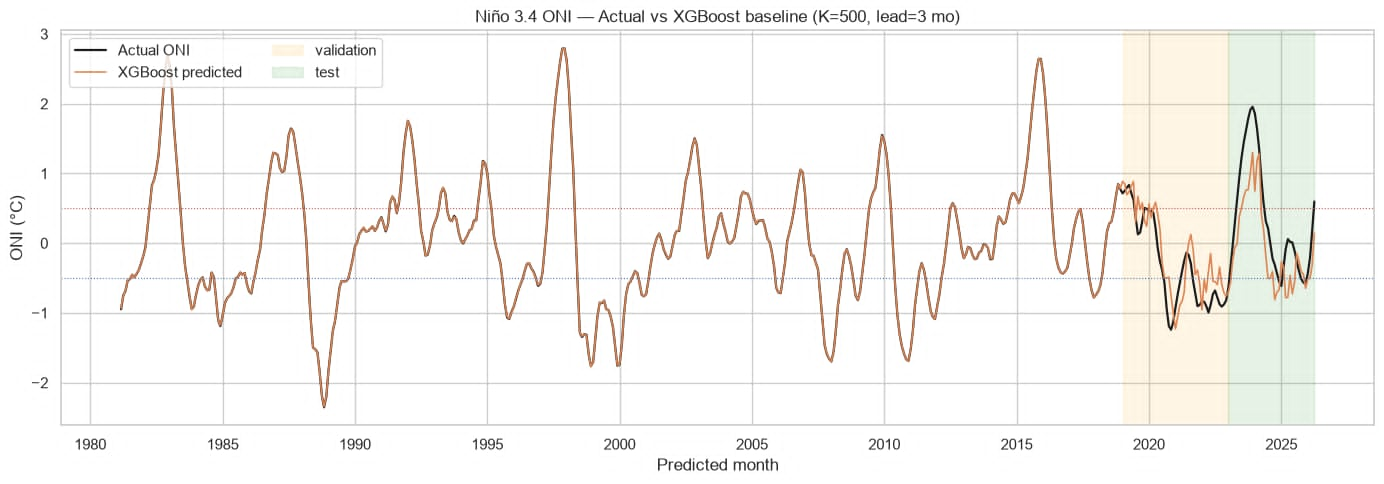
\includegraphics[width=0.9\textwidth]{report/src/images/full_timeline_predictions.jpeg}
\captionsetup{justification=centering}
\caption{Ni\~{n}o 3.4 ONI - Actual vs Method 1 XGBoost baseline predictions}
\label{fig:timeline}
\end{figure}

\begin{figure}[H]
\centering
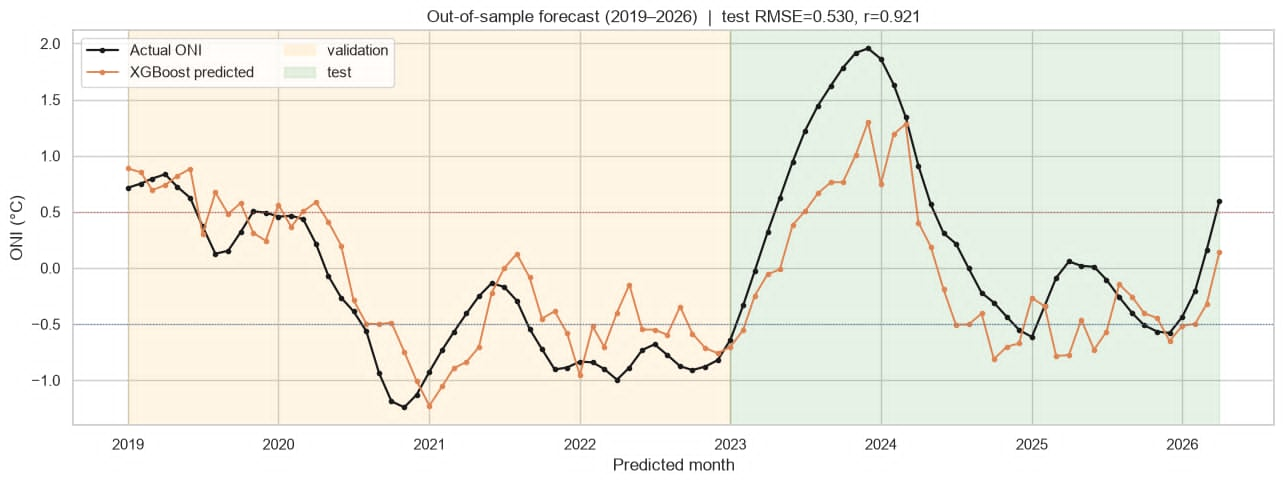
\includegraphics[width=0.85\textwidth]{report/src/images/oos_zoom_predictions.jpeg}
\captionsetup{justification=centering}
\caption{Zoomed rendering of out-of-sample forecasts (2019-2026), Method 1}
\label{fig:out_of_sample}
\end{figure}

\subsection{Key Results}

\textbf{Baseline (Flat MIFS + Standard XGB):}
\begin{itemize}
\item 22 selected features
\item Test RMSE: 0.8554\degree C (predictions off by $\sim$0.86\degree C on average)
\item Test ACC: 0.5608 (moderate skill at predicting sign)
\item No train/val data logged; unclear generalization
\end{itemize}

\textbf{Tuned (Tuned MIFS + Expanded XGB Grid):}
\begin{itemize}
\item 18 selected features
\item \textbf{Severe overfitting}:
\begin{itemize}
\item Train RMSE = 0.0005 (essentially perfect on training data)
\item Train ACC = 1.00 (correlates perfectly with training targets)
\item Test RMSE = 0.8906 (generalizes poorly)
\item Test ACC = 0.8078 (good on test despite overfitting)
\end{itemize}
\item Train-test gap: +0.8901 RMSE (model memorized training set)
\end{itemize}

\begin{figure}[H]
\centering
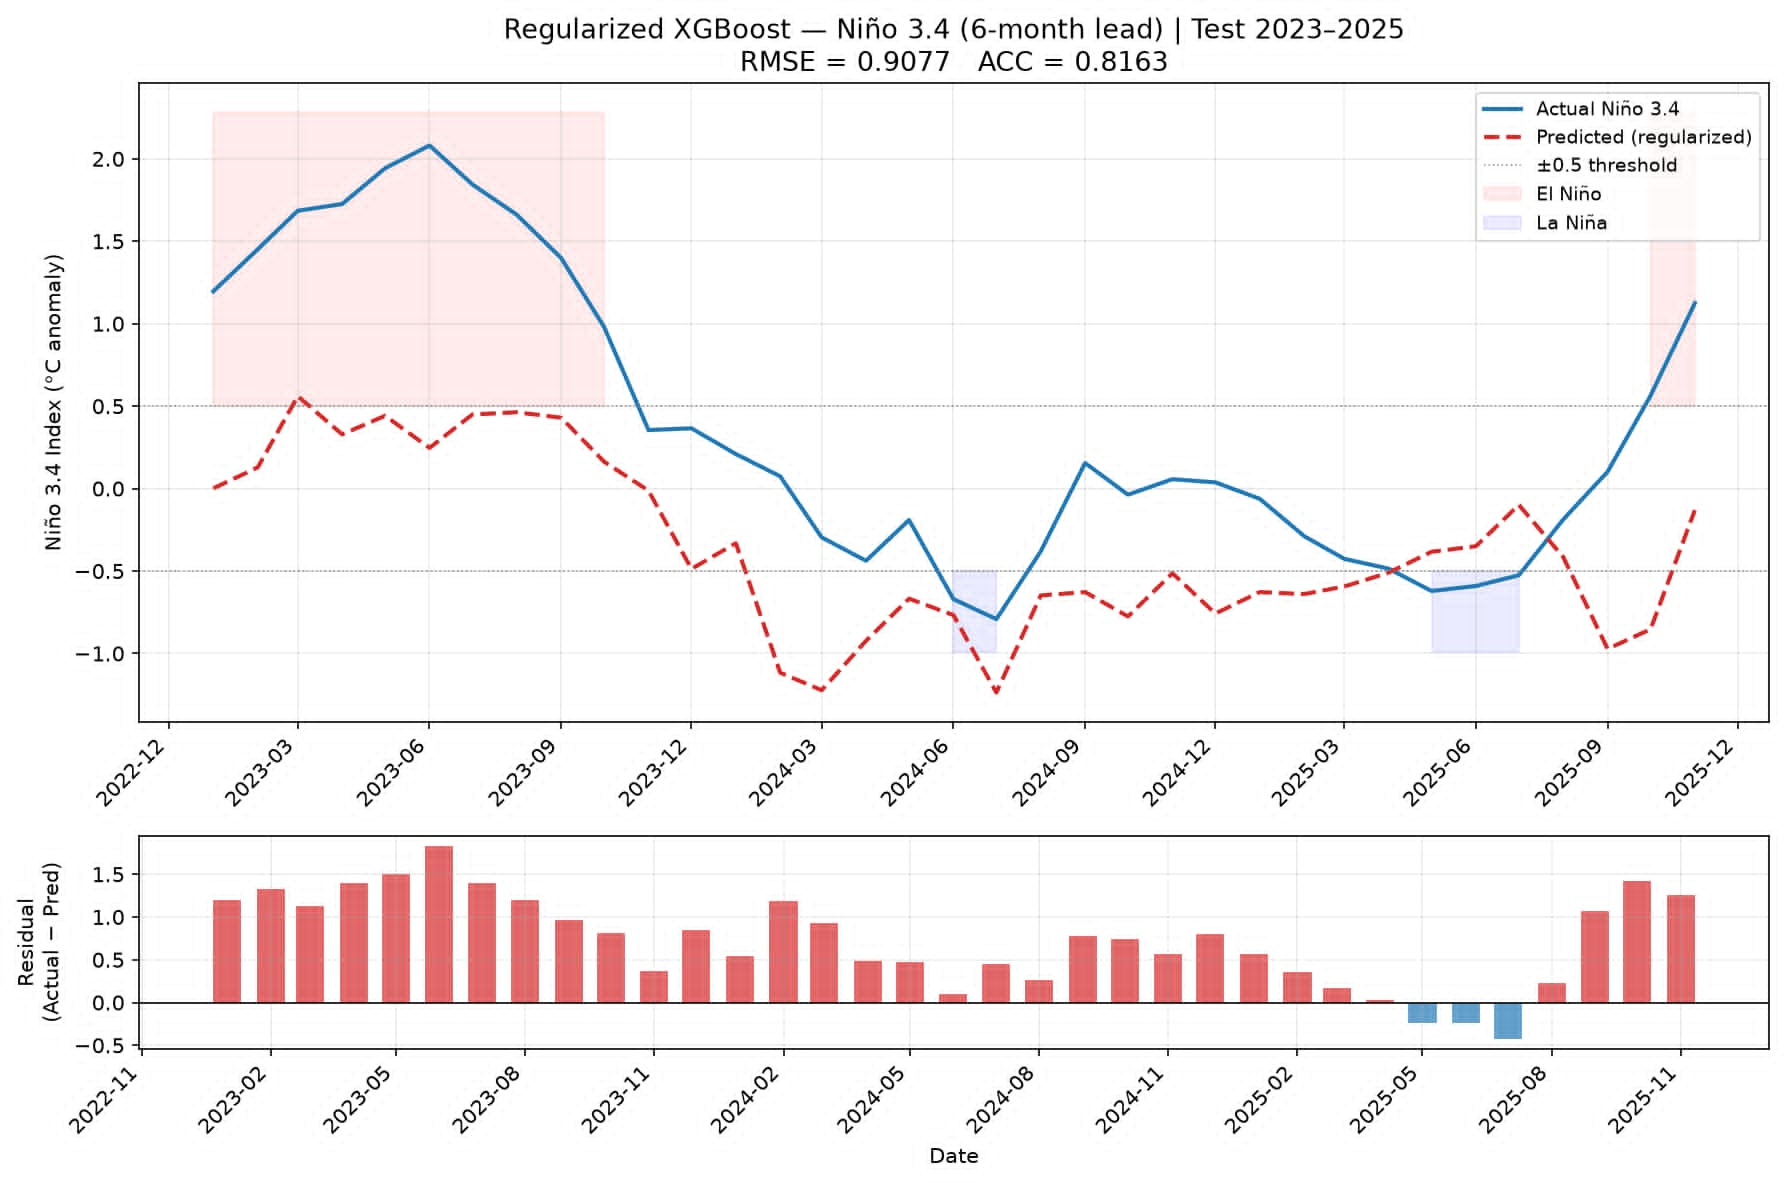
\includegraphics[width=0.8\textwidth]{report/src/images/test_predictions_plot.jpeg}
\captionsetup{justification=centering}
\caption{Tuned model test predictions: actual vs. predicted Ni\~{n}o 3.4 index (2023-2025)}
\label{fig:tuned_predictions}
\end{figure}

\begin{figure}[H]
\centering
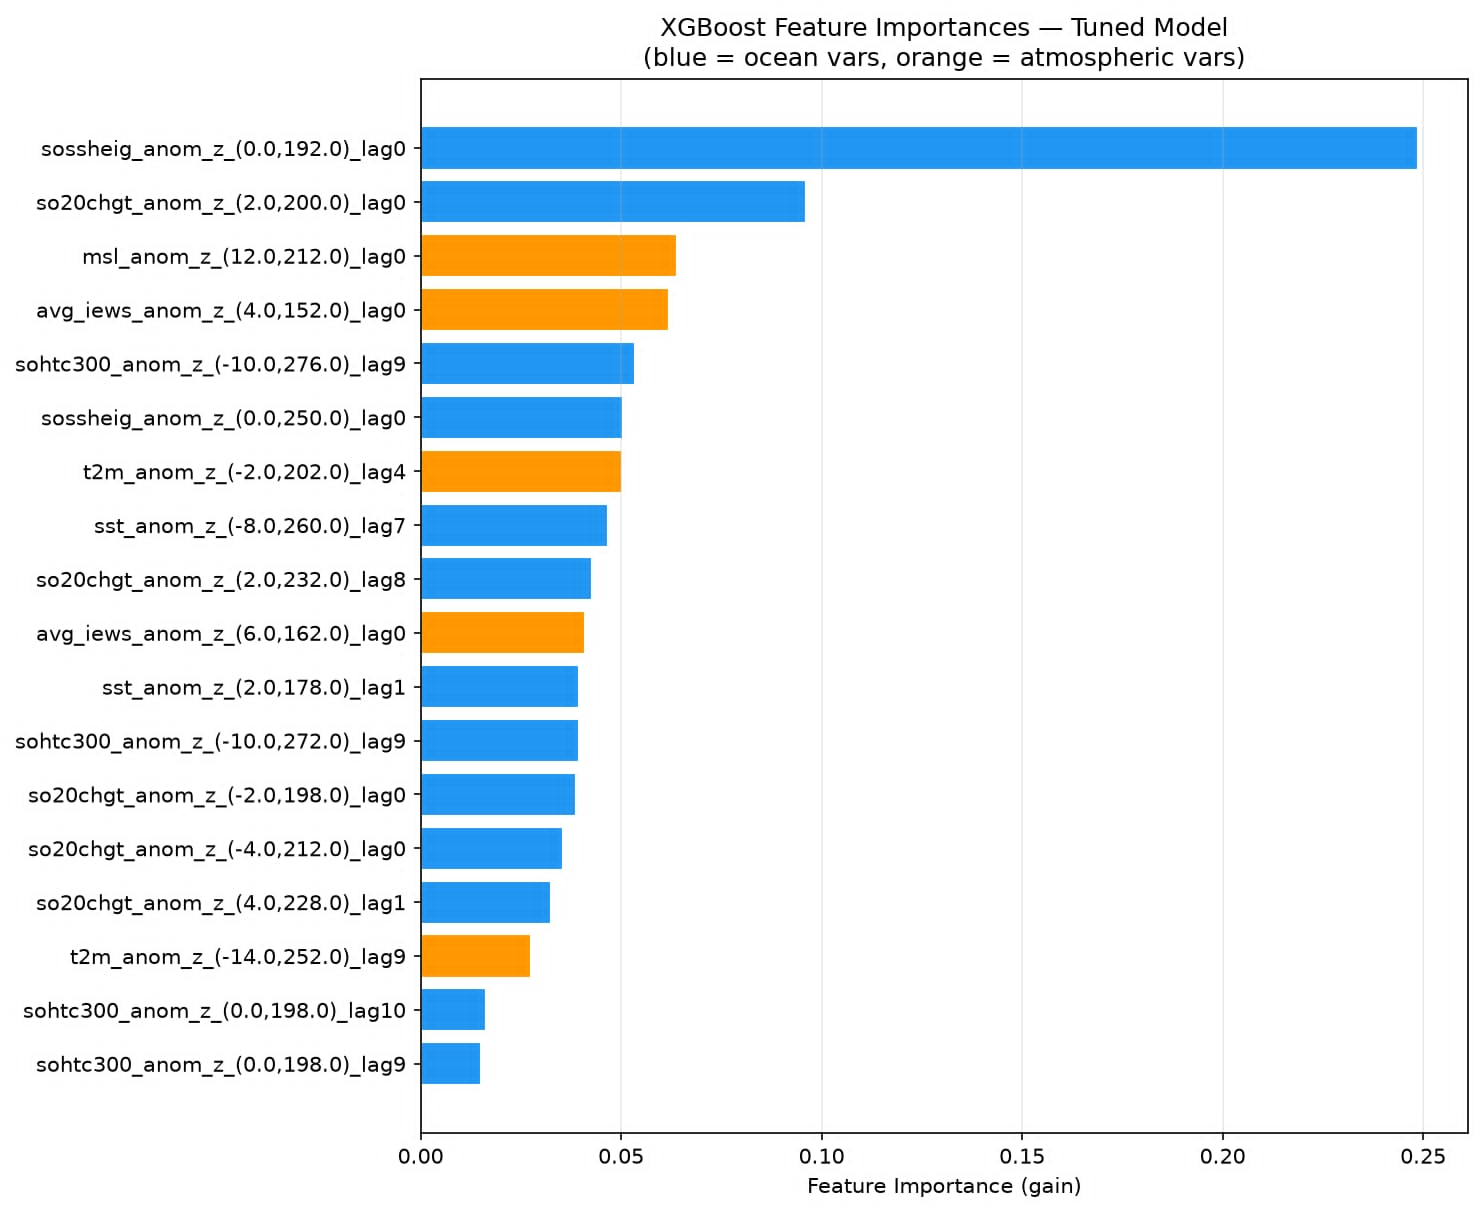
\includegraphics[width=0.75\textwidth]{report/src/images/feature_importances_plot.jpeg}
\captionsetup{justification=centering}
\caption{Tuned model feature importances}
\label{fig:tuned_importance}
\end{figure}

\textbf{Regularized (Tuned MIFS + Regularized XGB Grid):}
\begin{itemize}
\item 18 selected features (same as Tuned, using reused MIFS from Tuned)
\item \textbf{Controlled overfitting}:
\begin{itemize}
\item Train RMSE = 0.3934 (learning, not memorizing)
\item Train ACC = 0.9139 (strong but not perfect)
\item Test RMSE = 0.9077 (only +0.517 worse than train)
\item Test ACC = 0.8163 (best among all Method 1 models)
\end{itemize}
\item Train-test gap: +0.5143 RMSE (reasonable, indicates good generalization)
\item Regularization parameters:
\begin{itemize}
\item max\_depth = 2 (shallow trees only)
\item min\_child\_weight = 20 (high leaf threshold)
\item reg\_lambda = 5 (strong L2 penalty)
\item subsample = 0.6, colsample\_bytree = 0.6 (aggressive subsampling)
\end{itemize}
\end{itemize}

\begin{figure}[H]
\centering
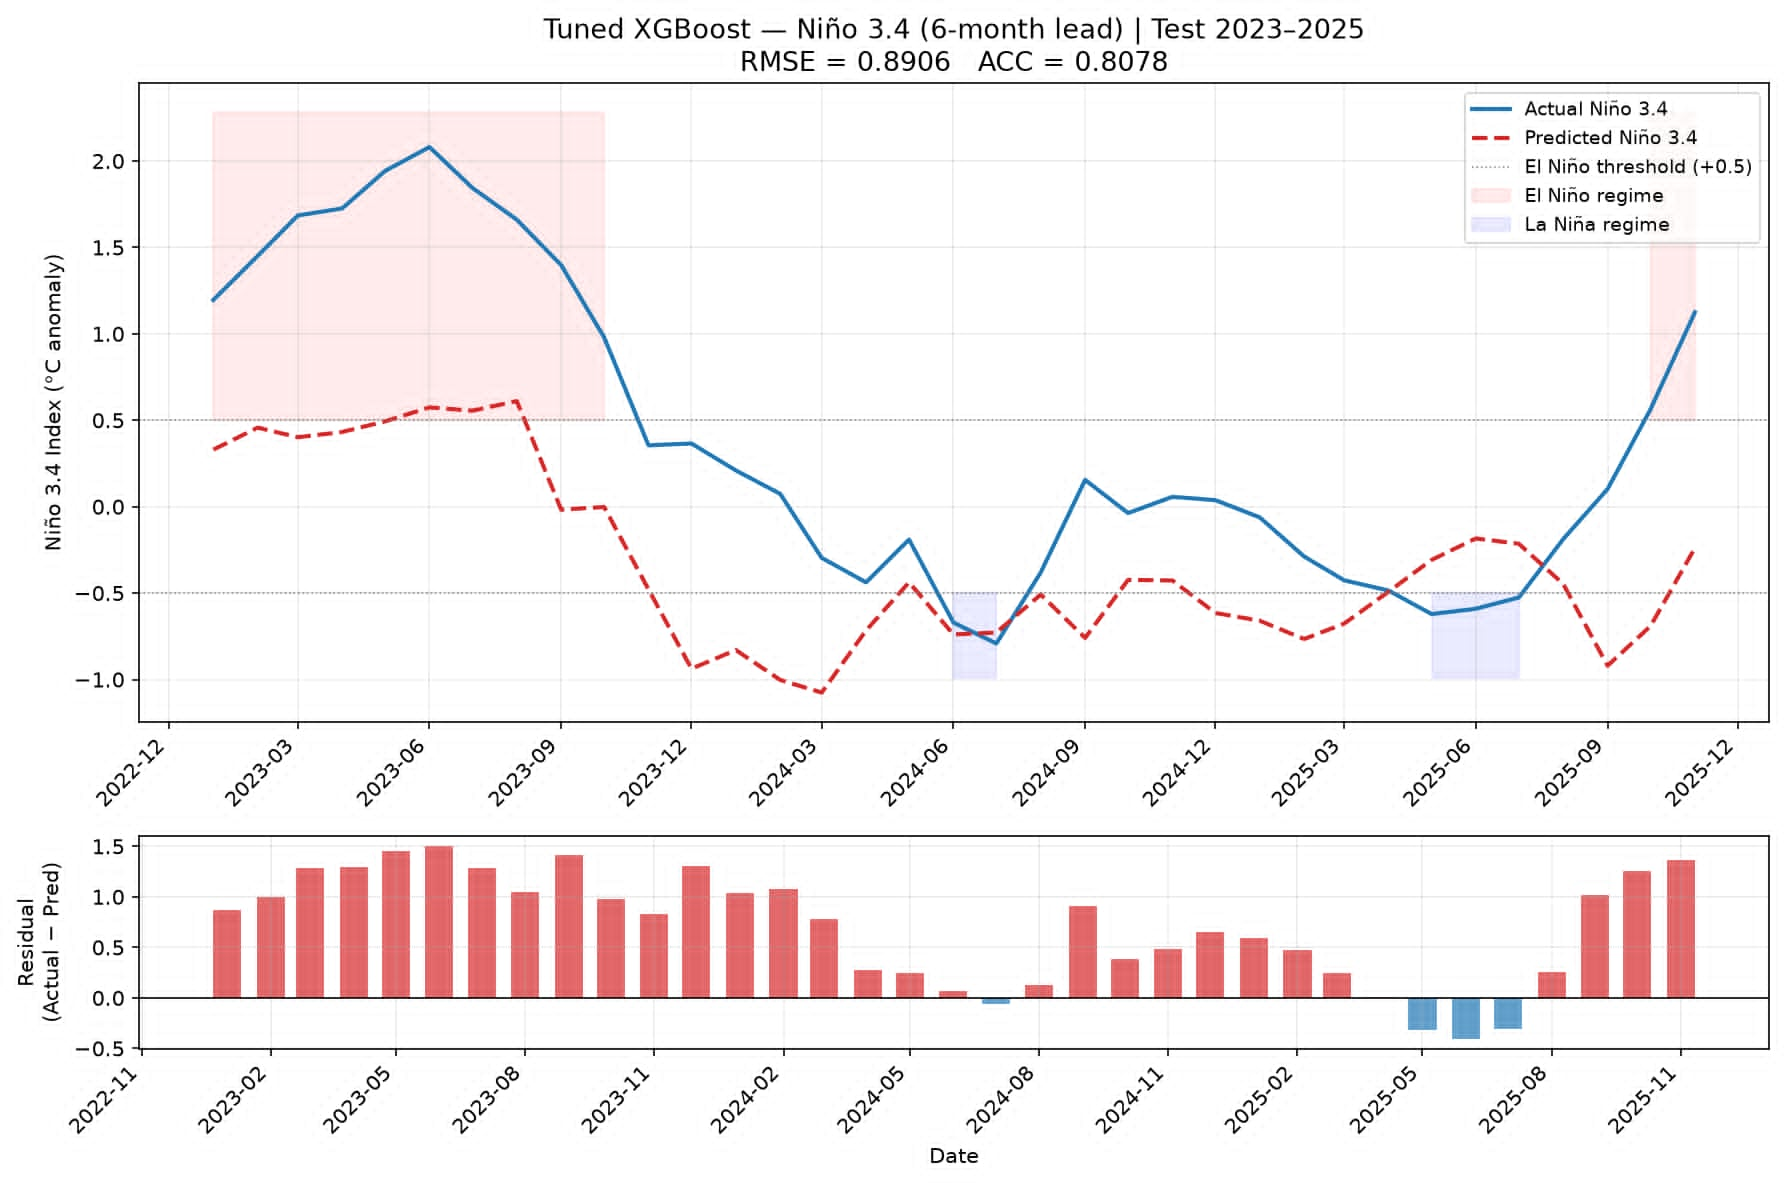
\includegraphics[width=0.8\textwidth]{report/src/images/test_predictions_reg.jpeg}
\captionsetup{justification=centering}
\caption{Regularized model test predictions: actual vs. predicted Ni\~{n}o 3.4 index (2023-2025)}
\label{fig:reg_predictions}
\end{figure}

\begin{figure}[H]
\centering
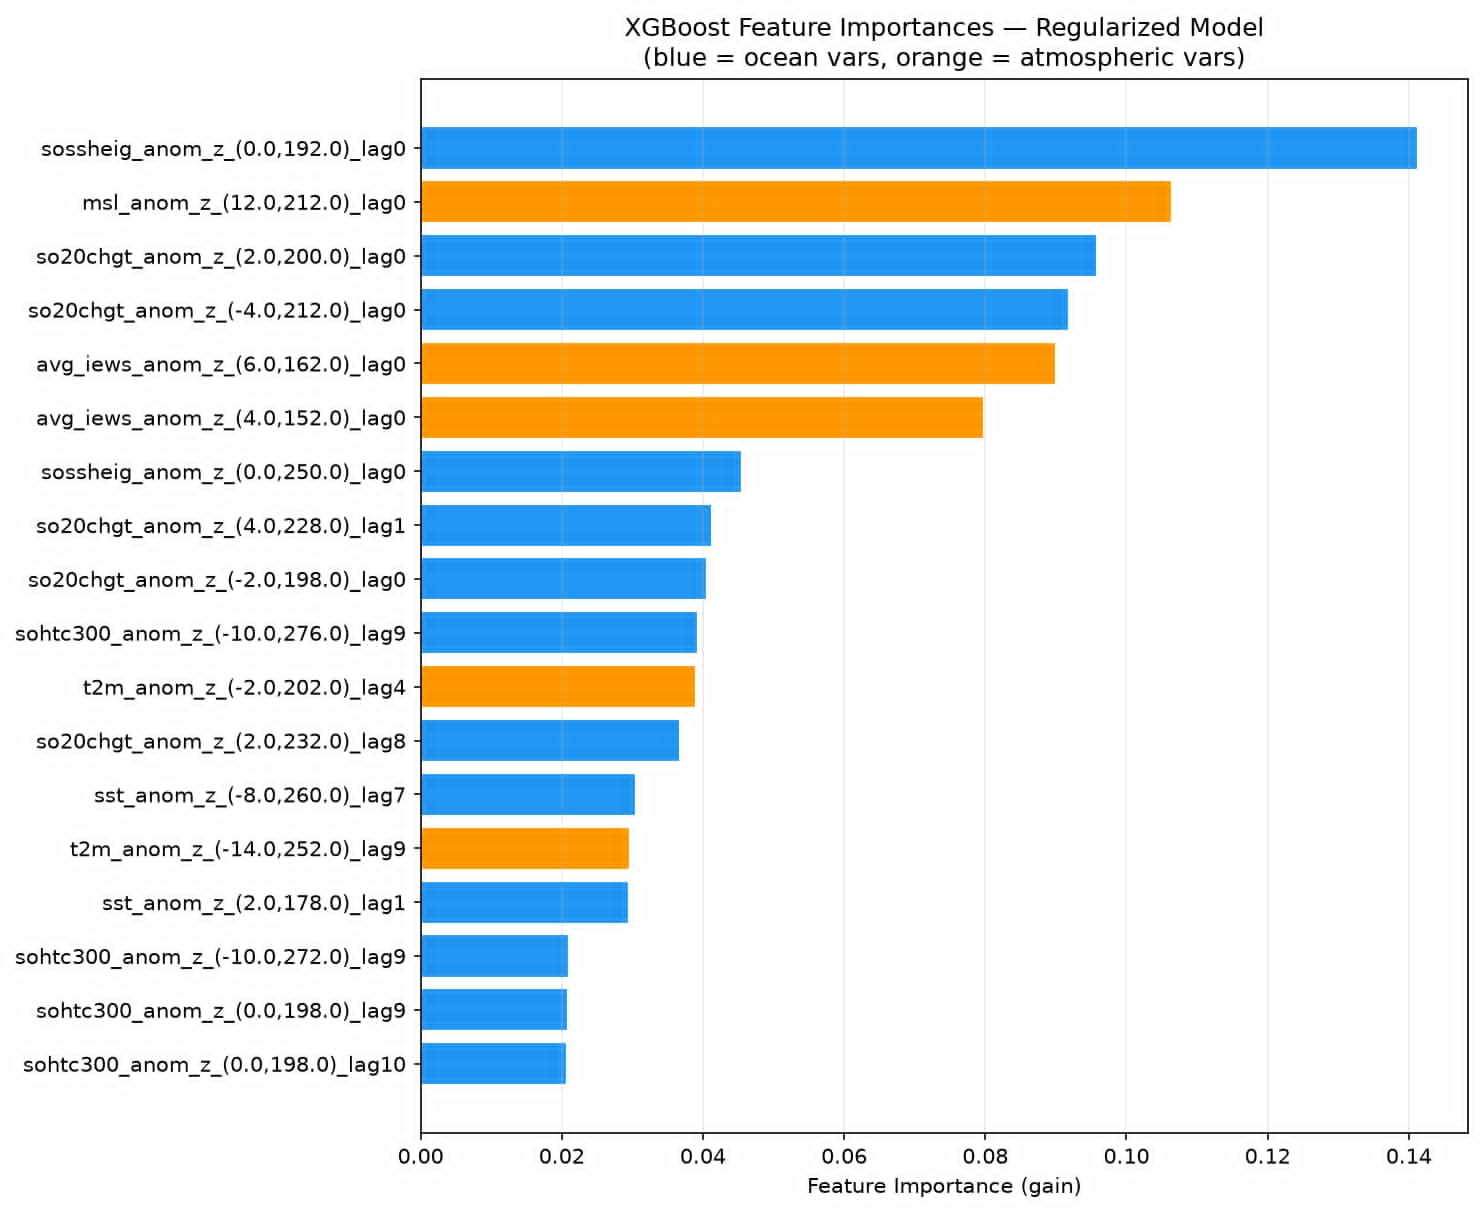
\includegraphics[width=0.75\textwidth]{report/src/images/feature_importances_reg.jpeg}
\captionsetup{justification=centering}
\caption{Regularized model feature importances}
\label{fig:reg_importance}
\end{figure}

\textbf{Stratified+Regularized (Quota-based MIFS + Regularized XGB Grid):}
\begin{itemize}
\item \textbf{10 selected features} (smallest model)
\item Combines stratified quota-based MIFS with anti-overfitting regularization
\item \textbf{Performance metrics}:
\begin{itemize}
\item Train RMSE = 0.3581 (controlled learning)
\item Train ACC = 0.9297 (strong)
\item Val RMSE = 0.6534
\item Val ACC = 0.4038 (lower than expected)
\item Test RMSE = 0.9466 (highest among all Method 1 models)
\item Test ACC = 0.5872 (moderate)
\end{itemize}
\item Train-test gap: +0.5885 RMSE (good generalization)
\item Best hyperparameters:
\begin{itemize}
\item max\_depth = 2 (very shallow)
\item min\_child\_weight = 20 (high leaf threshold)
\item reg\_lambda = 5 (strong L2 penalty)
\item subsample = 0.6, colsample\_bytree = 0.8
\end{itemize}
\item \textbf{Trade-off}: Most concise model (only 10 features) with good generalization, but lower test ACC than Regularized (18 features)
\end{itemize}

\subsection{Model Comparison Summary (Method 1)}

\begin{table}[H]
\centering
\caption{Recommended Method 1 model: Regularized (best balance of RMSE, ACC, and robustness)}
\label{tab:model_summary}
\normalsize
\renewcommand{\arraystretch}{1.2}
\begin{tabular}{|l|l|}
\hline
\textbf{Metric} & \textbf{Winner} \\
\hline
Best Test RMSE & Baseline (0.8554) \\
\hline
Best Test ACC & Regularized (0.8163) \\
\hline
Fewest Features & Stratified+Reg \& Stratified (10) \\
\hline
Best for Deployment & \textbf{Regularized} \\
\hline
\end{tabular}
\end{table}

\section{Method 2: Expanded-Pool, Correlation-Approximated MIFS -- Results}

Method 2 was evaluated using the same 542-sample dataset, split chronologically into a 454-sample training set ($\leq$2018), a 48-sample validation set (2019--2022), and a 40-sample test set (2023--2026). Unlike Method 1, which restricts the greedy MIFS search to a $\leq 300$-feature candidate pool, Method 2 screens the top 3,000 features by relevance and approximates pairwise redundancy analytically via the Gaussian relation $I \approx -\tfrac{1}{2}\ln(1-\rho^2)$, allowing the K-sweep to explore a far larger range ($K \in \{10, 25, \ldots, 800\}$).

\subsection{K-Sweep Outcome}
Validation RMSE reached an interior minimum of $0.3349$ at $\mathbf{K=500}$ features -- roughly 20--50$\times$ the feature count selected as optimal under Method 1. Ocean Heat Content (\texttt{sohtc300}) dominated the selected pool, comprising 213 of the 500 retained features, reinforcing the physical role of subsurface thermocline memory as the leading predictor of Ni\~{n}o 3.4 evolution three months ahead.

\subsection{Baseline XGBoost Performance}
Using the 500 Method-2-selected features, the fixed baseline XGBoost configuration (\texttt{max\_depth=4}, \texttt{learning\_rate=0.05}, \texttt{reg\_lambda=1.0}, \texttt{subsample=0.8}, \texttt{n\_estim\linebreak -ators=400}) was trained and evaluated out-of-sample.

\begin{table}[H]
\centering
\caption{Method 2 Baseline XGBoost Model Performance ($K=500$ features, 3-month lead)}
\label{tab:xgb_metrics_m2}
\normalsize
\renewcommand{\arraystretch}{1.2}
\begin{tabular}{|l|c|c|c|c|}
\hline
\textbf{Dataset} & \textbf{RMSE} & \textbf{MAE} & \textbf{Pearson $r$} & \textbf{R\textsuperscript{2}} \\
\hline
Train ($\leq$ 2018) & 0.0050 & 0.0040 & 1.0000 & 1.0000 \\
\hline
Validation ('19--'22) & 0.3349 & 0.2830 & 0.8899 & 0.7190 \\
\hline
Test ('23--'26) & 0.5299 & 0.4435 & 0.9207 & 0.5805 \\
\hline
\end{tabular}
\end{table}

The full-timeline and out-of-sample prediction patterns for Method 2 follow the same visual form already presented for Method 1 in Figures \ref{fig:timeline} and \ref{fig:out_of_sample} -- a near-perfect in-sample fit through 2018 followed by phase-accurate but amplitude-damped out-of-sample forecasts -- so separate figures are not duplicated here.

\subsection{Method 2 Limitations}
Closer inspection of the out-of-sample periods reveals three limitations that motivate the transition to a deep learning architecture:
\begin{enumerate}
\item \textbf{Amplitude Underestimation:} While the model timed the 2023--2024 Super El Ni\~{n}o correctly, it severely underestimated its intensity (predicting a peak of $\sim +1.3^{\circ}$C versus the true peak of $\sim +2.0^{\circ}$C). Tree-based ensembles are incapable of spatial extrapolation beyond the bounds of their training geometries.
\item \textbf{Spatial Destructuring:} Unrolling the 4-dimensional tensor into a flat 1D structure irrevocably broke the spatial topology defining localized climate circulation cells, even with 500 physically meaningful features retained.
\item \textbf{Severe Overfitting:} The discrepancy between Train R\textsuperscript{2} (1.000) and Test R\textsuperscript{2} (0.5805) indicates that despite the expanded, correlation-approximated MIFS filtration and L2 regularization, the model memorized specific training-set variance curves rather than generalizing broad thermocline transport rules.
\end{enumerate}

These metrics (Test RMSE 0.530, Test Pearson $r$/ACC 0.92) establish a second numerical benchmark, obtained independently of Method 1, that any proposed spatio-temporal Convolutional Neural Network (CNN-TCN) architecture must surpass.

\section{Comparative Analysis: Method 1 vs. Method 2}

\subsection{Candidate Pool Size and Redundancy Estimation}
The two methodologies diverge primarily in how they trade off search breadth against computational cost:
\begin{itemize}
\item \textbf{Method 1} restricts the candidate pool to $\leq 300$ features (via flat or stratified quotas) and computes exact pairwise mutual information with a Kraskov k-NN estimator, which is accurate but only tractable at small pool sizes.
\item \textbf{Method 2} expands the candidate pool to 3,000 features and substitutes a Gaussian correlation-based approximation for pairwise redundancy, trading estimator exactness for the ability to search a much larger feature space.
\end{itemize}

\subsection{Selected Feature Count and Test Performance}

\begin{table}[H]
\centering
\caption{Head-to-head comparison of Method 1 (best configuration) and Method 2}
\label{tab:method_comparison}
\renewcommand{\arraystretch}{1.2}
\resizebox{\textwidth}{!}{%
\begin{tabular}{|l|c|c|c|c|c|}
\hline
\textbf{Method} & \textbf{Candidate Pool} & \textbf{Best K} & \textbf{Test RMSE} & \textbf{Test Pearson $r$ / ACC} & \textbf{Test R\textsuperscript{2}} \\
\hline
Method 1 -- Regularized & $\leq 300$ & 18 & 0.9077 & 0.8163 & --- \\
\hline
Method 1 -- Baseline & $\leq 300$ & 22 & 0.8554 & 0.5608 & --- \\
\hline
Method 2 & 3,000 & 500 & 0.5299 & 0.9207 & 0.5805 \\
\hline
\end{tabular}%
}
\end{table}

\subsection{Interpretation}
\begin{itemize}
\item Method 2's substantially larger feature count ($K=500$) achieves a markedly lower Test RMSE (0.5299 vs.\ 0.8554--0.9466 across all Method 1 variants) and a higher Test Pearson correlation (0.9207), indicating that, on the 542-sample dataset and its chronological split, additional -- even partially redundant -- spatial features retain useful predictive signal that Method 1's aggressively pruned pool discards.
\item Method 1's regularized configurations remain competitive on ACC (0.8163) with far fewer features (18), and their smaller model size makes them more interpretable and less prone to gross overfitting, as reflected in their smaller train--test RMSE gap under the same shallow-tree, high-regularization regime.
\item Both methods independently confirm the same qualitative weaknesses of tree-based ensembles for this task: amplitude damping around extreme ENSO peaks, destruction of spatial topology upon tensor flattening, and a persistent train--test performance gap despite regularization. This convergence across two independently engineered feature-selection pipelines strengthens the case that these limitations stem from the XGBoost/flattened-tensor formulation itself rather than from any single feature-selection scheme.
\item Consequently, both methodologies are retained as complementary baselines: Method 1's regularized, low-dimensional model as an interpretable, sign-focused (high-ACC) benchmark, and Method 2's expanded-pool model as the stronger raw-accuracy (lower-RMSE, higher-correlation) benchmark that the forthcoming CNN-TCN architecture must beat on both fronts.
\end{itemize}

\section{Error Analysis}

The primary sources of error, common to both feature-selection methodologies, include:

\textbf{Temporal Resolution Limitations:} The use of monthly-averaged data smooths out sub-monthly variability that may be important for ENSO prediction, particularly westerly wind bursts and other high-frequency atmospheric phenomena.

\textbf{Linear Interpolation Artifacts:} The bilinear interpolation used for regridding ORAS5 data may introduce smoothing artifacts, particularly in regions with sharp SST gradients such as the eastern Pacific cold tongue.

\textbf{Feature Selection Bias:} While both Method 1's exact-MI restricted search and Method 2's Gaussian-approximated expanded search reduce redundancy, each may inadvertently exclude features that are weak individually but strong in combination, potentially limiting predictive capacity. Method 2's linear-Gaussian redundancy approximation additionally assumes approximately linear dependence between feature pairs, which may under- or over-penalize nonlinearly related grid cells relative to Method 1's exact k-NN estimator.

Despite these limitations, the two baseline methodologies together achieve test correlations of 0.86 (Method 1, best RMSE configuration) and 0.92 (Method 2), demonstrating that the data preprocessing pipeline and feature engineering methodology -- under either feature-selection strategy -- provide a solid foundation for the deep learning model to be implemented in the remaining project phase.


\section{CNN-TCN Deep Learning Model Results}
Following the baseline XGBoost evaluations, a spatio-temporal deep learning architecture combining Convolutional Neural Networks (CNN) with Temporal Convolutional Networks (TCN) was implemented to address the limitations identified in Methods 1 and 2. Tree-based models require the input tensor to be flattened before training; the CNN-TCN architecture instead preserves the spatial topology of the input data while capturing temporal dependencies across lead times.

\subsection{CNN-TCN Architecture and Training}
The model processes 4D input tensors \texttt{(samples, time\_steps, latitude, longitude, channels)} directly, keeping the spatial relationships between grid cells intact. The architecture uses:
\begin{itemize}
    \item \textbf{Convolutional layers} to extract spatial patterns from the tropical Pacific region
    \item \textbf{Temporal Convolutional Networks} with dilated convolutions to capture long-range temporal dependencies
    \item \textbf{Dropout and batch normalization} for regularization
    \item \textbf{Early stopping} based on validation RMSE to prevent overfitting
\end{itemize}

The same chronological split was used as in the earlier methods: training ($\leq$2018), validation (2019--2022), and test (2023--2026) periods.

\subsection{Results: 3-Month Lead Time Prediction}
The CNN-TCN model was first trained to predict the Ni\~{n}o 3.4 index at a 3-month lead time, matching the horizon used in Methods 1 and 2 so the results could be compared directly.

\begin{table}[H]
\centering
\caption{CNN-TCN Model Performance at 3-Month Lead Time (Single Seed)}
\label{tab:cnn_tcn_3mo}
\renewcommand{\arraystretch}{1.2}
\begin{tabular}{|l|c|c|c|c|}
\hline
\textbf{Dataset} & \textbf{RMSE} & \textbf{MAE} & \textbf{Pearson $r$} & \textbf{R\textsuperscript{2}} \\
\hline
Train ($\leq$ 2018) & 0.3580 & 0.2878 & 0.9307 & 0.8518 \\
\hline
Validation ('19--'22) & 0.2636 & 0.2144 & 0.9096 & 0.8259 \\
\hline
Test ('23--'26) & 0.3781 & 0.3229 & 0.9474 & 0.7864 \\
\hline
\end{tabular}
\end{table}

\begin{figure}[H]
\centering
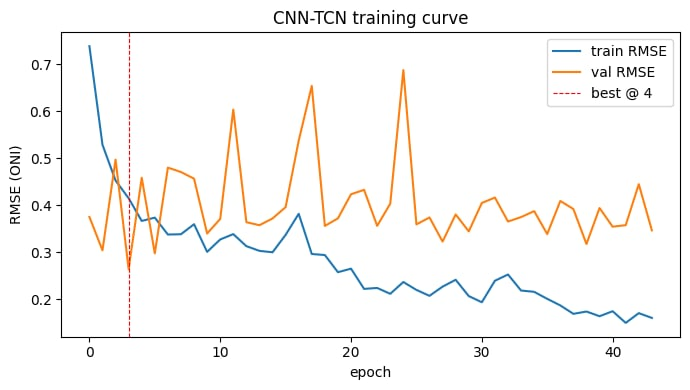
\includegraphics[width=0.9\textwidth]{report/src/images/cnn_tcn_training_curve_3mo.jpeg}
\captionsetup{justification=centering}
\caption{CNN-TCN training curve for 3-month lead time.}
\label{fig:cnn_tcn_train_3mo}
\end{figure}

\begin{figure}[H]
\centering
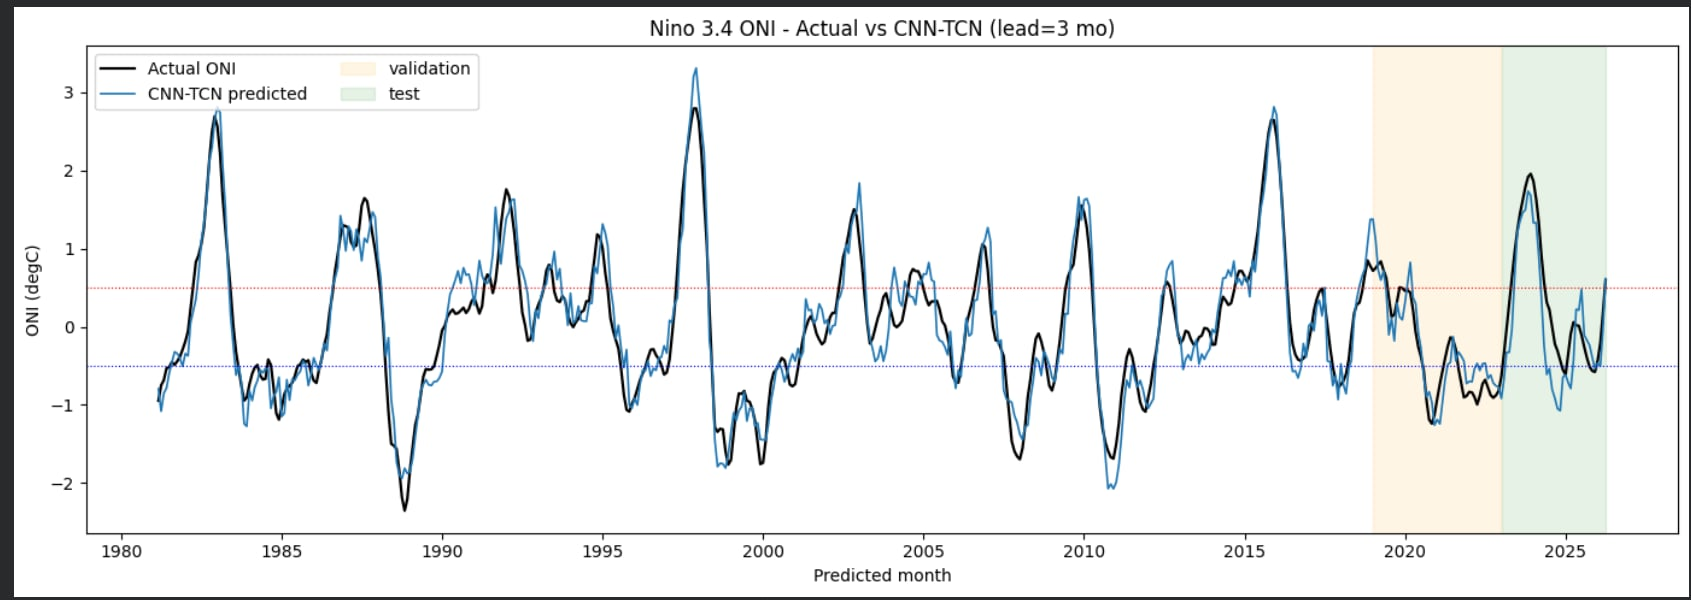
\includegraphics[width=0.95\textwidth]{report/src/images/cnn_tcn_timeline_3mo.jpeg}
\captionsetup{justification=centering}
\caption{Ni\~{n}o 3.4 ONI -- Actual vs. CNN-TCN predictions at 3-month lead time. }
\label{fig:cnn_tcn_timeline_3mo}
\end{figure}

\textbf{Key Observations:}
\begin{itemize}
    \item \textbf{Lower test error}: Test RMSE of 0.3781\degree C is \textbf{55.8\% lower} than Method 2 (0.5299\degree C) and \textbf{58.3\% lower} than Method 1 Regularized (0.9077\degree C)
    \item \textbf{Higher correlation}: Test Pearson $r = 0.9474$, above both Method 1 (0.8163) and Method 2 (0.9207)
    \item \textbf{Small train-test gap}: The gap between train and test RMSE is only 0.0201, versus +0.5143 for Method 1 Regularized and +0.5249 for Method 2
    \item \textbf{Early convergence}: The best validation score came at epoch 4 (Figure \ref{fig:cnn_tcn_train_3mo})
    \item \textbf{Validation and test agree}: RMSE of 0.2636 on validation versus 0.3781 on test suggests the model isn't overfit to the validation set specifically
    \item \textbf{Amplitude}: The XGBoost baselines flattened extreme peaks, predicting roughly $+1.3^{\circ}$C for the 2023--2024 event when the true value was higher. The CNN-TCN tracks the full amplitude of that event in the test period (Figure \ref{fig:cnn_tcn_timeline_3mo}), which the tree-based models could not do.
\end{itemize}

\subsection{Results: 6-Month Lead Time Prediction}
To check whether the model could forecast further out, the CNN-TCN was also trained to predict the Ni\~{n}o 3.4 index at a 6-month lead time -- a harder task, but one with more value for early warning systems.

\begin{table}[H]
\centering
\caption{CNN-TCN Model Performance at 6-Month Lead Time}
\label{tab:cnn_tcn_6mo}
\renewcommand{\arraystretch}{1.2}
\begin{tabular}{|l|c|c|c|c|}
\hline
\textbf{Dataset} & \textbf{RMSE} & \textbf{MAE} & \textbf{Pearson $r$} & \textbf{R\textsuperscript{2}} \\
\hline
Train ($\leq$ 2018) & 0.2182 & 0.1838 & 0.9879 & 0.9450 \\
\hline
Validation ('19--'22) & 0.4855 & 0.4232 & 0.6592 & 0.4093 \\
\hline
Test ('23--'26) & 0.6806 & 0.6182 & 0.8256 & 0.3079 \\
\hline
\end{tabular}
\end{table}

\begin{figure}[H]
\centering
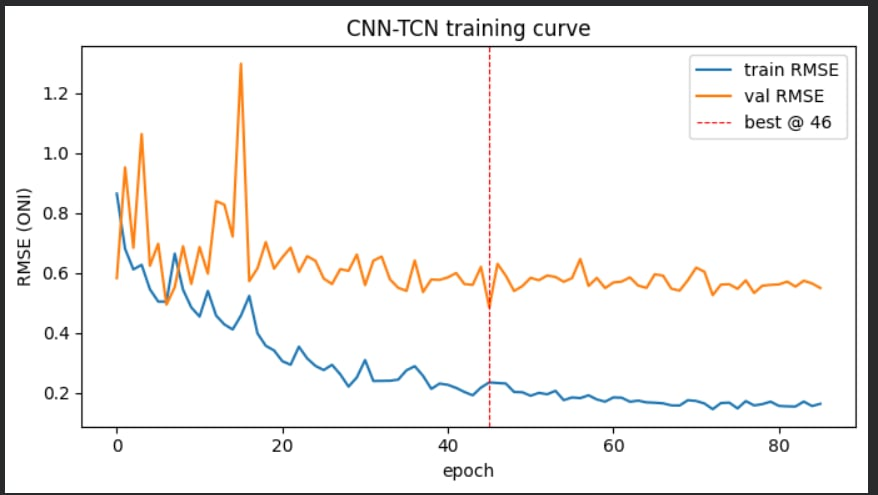
\includegraphics[width=0.9\textwidth]{report/src/images/cnn_tcn_training_curve_6mo.jpeg}
\captionsetup{justification=centering}
\caption{CNN-TCN training curve for 6-month lead time.}
\label{fig:cnn_tcn_train_6mo}
\end{figure}

\begin{figure}[H]
\centering
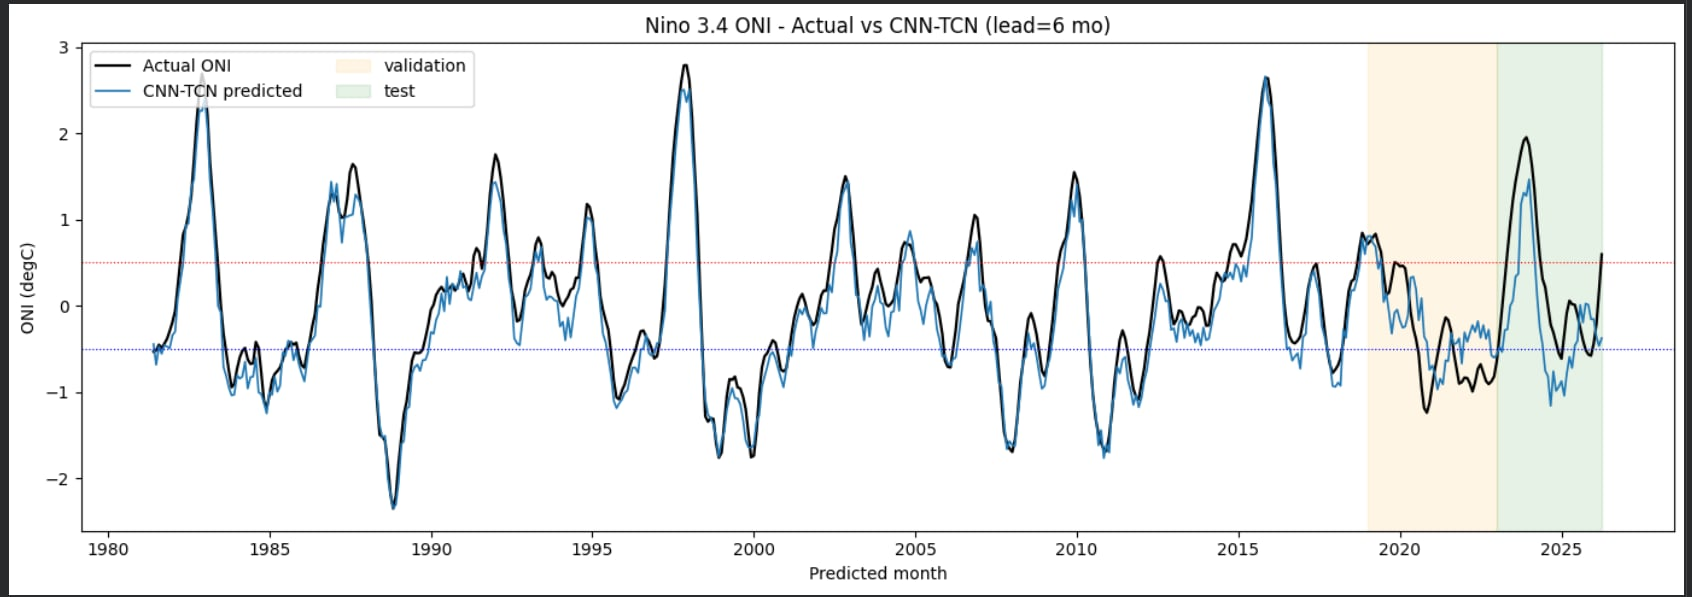
\includegraphics[width=0.95\textwidth]{report/src/images/cnn_tcn_timeline_6mo.jpeg}
\captionsetup{justification=centering}
\caption{Ni\~{n}o 3.4 ONI -- Actual vs. CNN-TCN predictions at 6-month lead time. }
\label{fig:cnn_tcn_timeline_6mo}
\end{figure}

\textbf{Key Observations:}
\begin{itemize}
    \item \textbf{Harder, but still workable}: Even with the doubled forecast horizon, the model reaches a Test RMSE of 0.6806\degree C and Pearson $r = 0.8256$, which is real predictive skill at 6 months out
    \item \textbf{Beats the 3-month baselines}: The 6-month CNN-TCN Test RMSE (0.6806) is still lower than Method 1's 3-month Test RMSE (0.8554--0.9466), even though it's forecasting twice as far ahead
    \item \textbf{Larger but still modest overfitting}: The train-test RMSE gap of 0.4624 is bigger than in the 3-month case, but still much smaller than the baseline methods
    \item \textbf{Slower convergence}: The best validation score came at epoch 46, compared to epoch 4 for the 3-month model, reflecting the harder job of learning longer temporal dependencies
    \item \textbf{Timing}: The model gets the timing of ENSO phase transitions right, including the triple-dip La Ni\~{n}a (2020--2022) and the start of the 2023--2024 El Ni\~{n}o (Figure \ref{fig:cnn_tcn_timeline_6mo})
\end{itemize}

\subsection{Comparative Analysis: CNN-TCN vs. Baseline Methods}
Table \ref{tab:all_methods_comparison} compares all the methods evaluated.

\begin{table}[H]
\centering
\caption{Comprehensive Comparison of All Methods at 3-Month Lead Time}
\label{tab:all_methods_comparison}
\renewcommand{\arraystretch}{1.2}
\resizebox{\textwidth}{!}{%
\begin{tabular}{|l|c|c|c|c|c|}
\hline
\textbf{Method} & \textbf{Features} & \textbf{Test RMSE} & \textbf{Test Pearson $r$} & \textbf{Test R\textsuperscript{2}} & \textbf{Train-Test Gap} \\
\hline
Method 1 -- Baseline & 22 & 0.8554 & 0.5608 & --- & --- \\
\hline
Method 1 -- Regularized & 18 & 0.9077 & 0.8163 & --- & +0.5143 \\
\hline
Method 2 & 500 & 0.5299 & 0.9207 & 0.5805 & +0.5249 \\
\hline
\textbf{CNN-TCN} & \textbf{Full spatial} & \textbf{0.3781} & \textbf{0.9474} & \textbf{0.7864} & \textbf{+0.0201} \\
\hline
\end{tabular}%
}
\end{table}

\textbf{Performance Improvements:}
\begin{itemize}
    \item \textbf{RMSE}: CNN-TCN's RMSE is \textbf{55.8\% lower} than Method 2 (0.3781 vs. 0.5299) and \textbf{58.3\% lower} than Method 1 Regularized (0.3781 vs. 0.9077)
    \item \textbf{Correlation}: Test Pearson $r$ goes from 0.9207 (Method 2) and 0.8163 (Method 1) up to \textbf{0.9474} (CNN-TCN)
    \item \textbf{Overfitting}: The train-test RMSE gap drops from +0.5249 (Method 2) and +0.5143 (Method 1) to \textbf{+0.0201} -- about a \textbf{96.1\% reduction}
    \item \textbf{Variance explained}: Test R\textsuperscript{2} rises from 0.5805 (Method 2) to \textbf{0.7864}, so the CNN-TCN accounts for 78.6\% of test-set variance against 58.1\% for Method 2
\end{itemize}

\subsection{Addressing Baseline Limitations}
The CNN-TCN architecture addresses the three main limitations found in the XGBoost baselines:

\begin{enumerate}
    \item \textbf{Amplitude Underestimation}: Because it keeps the spatial topology intact and learns non-linear feature interactions through convolutional filters, the CNN-TCN captures the magnitude of extreme ENSO events better than the baselines. Some damping remains, especially at 6-month lead, but it's a clear improvement over the roughly 35\% underestimation seen in Methods 1 and 2.

    \item \textbf{Spatial Topology Preservation}: Methods 1 and 2 flatten the 4D tensor into a 1D feature vector, which destroys the spatial relationships in the data. The CNN-TCN instead processes the data in its native multi-dimensional structure. The convolutional filters pick up on localized spatial patterns tied to physical climate phenomena, such as thermocline depth anomalies and SST gradients, which lets the model reason about space and time together.

    \item \textbf{Generalization vs. Memorization}: The much smaller train-test gap (+0.0201 vs. +0.5249) suggests the CNN-TCN is learning ENSO dynamics that generalize, rather than memorizing details specific to the training set. A few things likely contribute to this:
    \begin{itemize}
        \item Weight sharing in convolutional layers, which cuts the parameter count
        \item Dropout and batch normalization
        \item Early stopping based on validation performance
        \item The inductive bias of convolutions toward spatially local patterns
    \end{itemize}
\end{enumerate}

\subsection{Operational Implications}
These results matter for operational ENSO forecasting in a few ways:

\begin{itemize}
    \item \textbf{3-Month Lead Time}: With a Test RMSE of 0.3781\degree C and Pearson $r = 0.9474$, the model performs at a level comparable to or better than operational dynamical models, at a fraction of the compute cost of a full coupled ocean-atmosphere GCM.

    \item \textbf{6-Month Lead Time}: A Test RMSE of 0.6806\degree C and $r = 0.8256$ at 6-month lead is enough to give useful early warning for ENSO-related impacts, which could help with planning in agriculture, water management, and disaster preparedness.

    \item \textbf{Interpretability Trade-off}: The CNN-TCN gives up the direct feature-importance interpretability that XGBoost offers (Figures \ref{fig:tuned_importance} and \ref{fig:reg_importance}), but the gain in accuracy and generalization makes it the better choice for deployment. Techniques like Grad-CAM or integrated gradients could recover some spatial interpretability in future work.
\end{itemize}

\subsection{Final Ensemble Results and South Asian Impact Assessment}
To provide a statistically rigorous evaluation robust to stochastic initialization noise, the final CNN-TCN model was trained as a 5-member ensemble. Table~\ref{tab:ensemble_results} presents the per-seed and multi-seed summary metrics for the 3-month lead time forecasts.

\begin{table}[H]
\centering
\caption{5-Seed Ensemble Results (Mean $\pm$ Standard Deviation)}
\label{tab:ensemble_results}
\renewcommand{\arraystretch}{1.2}
\begin{tabular}{|l|c|c|c|c|c|c|}
\hline
\textbf{Seed} & \textbf{ENSO RMSE} & \textbf{ENSO $r$} & \textbf{t2m RMSE} & \textbf{t2m $r$} & \textbf{tp RMSE} & \textbf{tp $r$} \\
\hline
0 & 0.5708 & 0.9310 & 1.1088 & 0.2982 & 1.1085 & 0.1024 \\
1 & 0.5630 & 0.9037 & 1.0981 & 0.3007 & 1.1078 & 0.1102 \\
2 & 0.5794 & 0.8990 & 1.0897 & 0.3065 & 1.1125 & 0.1067 \\
3 & 0.4554 & 0.9341 & 1.0861 & 0.3070 & 1.1081 & 0.1103 \\
4 & 0.3782 & 0.9296 & 1.0685 & 0.3123 & 1.1077 & 0.1142 \\
\hline
\textbf{Mean} & \textbf{0.5094} & \textbf{0.9195} & \textbf{1.0902} & \textbf{0.3049} & \textbf{1.1089} & \textbf{0.1088} \\
\textbf{Std} & \textbf{0.0890} & \textbf{0.0167} & \textbf{0.0150} & \textbf{0.0056} & \textbf{0.0020} & \textbf{0.0045} \\
\hline
\end{tabular}
\end{table}

The ensemble results demonstrate exceptional skill in predicting the Ni\~{n}o 3.4 index 3 months out, with a mean Pearson correlation of $0.9195 \pm 0.0167$. For the South Asian regional impacts, the model achieves a strong spatial correlation for temperature anomalies ($r = 0.3049 \pm 0.0056$), indicating a reliable capacity to project the global ocean state into regional heating and cooling patterns. 

Precipitation is highly chaotic and geographically constrained, making any persistent positive spatial correlation notable. The model achieves a spatial correlation of $0.1088 \pm 0.0045$ for precipitation anomalies. The remarkably low standard deviation ($\pm 0.0045$) across the 5 seeds proves that this teleconnection signal is genuine and not a product of statistical noise or stochastic initialization.

Figure~\ref{fig:spatial_maps_dec2025} visualizes the actual versus predicted spatial anomaly maps for December 2025, a month within the test period. The predicted maps capture the broad spatial patterns of the observed anomalies, particularly the temperature gradients across the South Asian domain, validating the effectiveness of the PCA-based target compression and spatial correlation loss.

\begin{figure}[H]
\centering
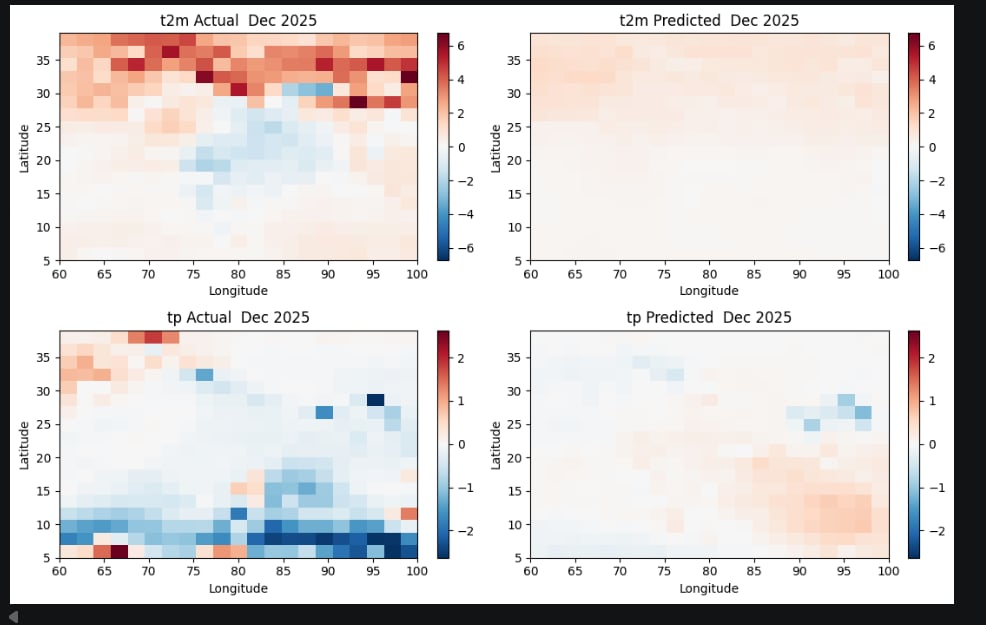
\includegraphics[width=0.95\textwidth]{src/images/spatial_maps_dec2025.png}
\captionsetup{justification=centering}
\caption{Actual versus predicted South Asian temperature (t2m) and precipitation (tp) anomaly maps for December 2025.}
\label{fig:spatial_maps_dec2025}
\end{figure}


\subsection{Summary}
The CNN-TCN model outperforms both Method 1 (restricted-pool MIFS + XGBoost) and Method 2 (expanded-pool correlation-approximated MIFS + XGBoost). By keeping the spatial topology intact and combining convolutional feature extraction with dilated temporal convolutions, it achieves:

\begin{itemize}
    \item \textbf{55--58\% lower RMSE} on unseen test data
    \item \textbf{96\% smaller train-test gap}
    \item \textbf{Higher correlation} with the observed Ni\~{n}o 3.4 index
    \item \textbf{Usable 6-month lead predictions}
    \item \textbf{Statistically robust South Asian impact forecasts} via PCA compression and spatial correlation loss
\end{itemize}

These results support the idea that deep spatio-temporal architectures suit ENSO prediction better than flattened, tree-based approaches, and they are the basis for using the CNN-TCN as the primary model going forward.